%!TEX root = ../bomberchamp.tex

Having introduced our minigame in \ref{ch:minigame}, we tried different network architectures to see what is necessary for an arena of size $(17, 17)$.
We chose a simple fully connected network with different numbers of neurons (Figure \ref{fig:dense-arch}) for our first tests and expanded on it with the convolutional network that was used on the Atari 2600 benchmark in the Rainbow DQN paper\cite{Hessel2018RainbowCI} (Figure \ref{fig:conv-original}). Since the input for the Atari benchmark was raw pixels with $w=h=84$, this might not be suitable for our problem with meaningful inputs of size $w=h=17$. So we modified the convolutional network to mimick the dimensions of the different layers of the original (Figure \ref{fig:conv-modified}).



\begin{figure}
  \centering
  \begin{subfigure}[b]{0.48\linewidth}
    \centering
    	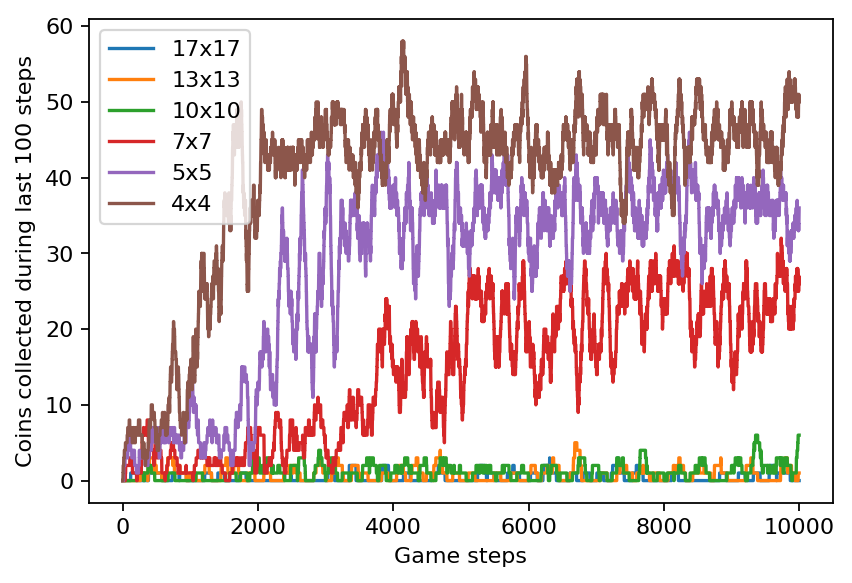
\includegraphics[width=\linewidth]{images/minigame-dense64-arch.png}
    \caption{Dense 64}
  \end{subfigure}
  \quad
  \begin{subfigure}[b]{0.48\linewidth}
    \centering
      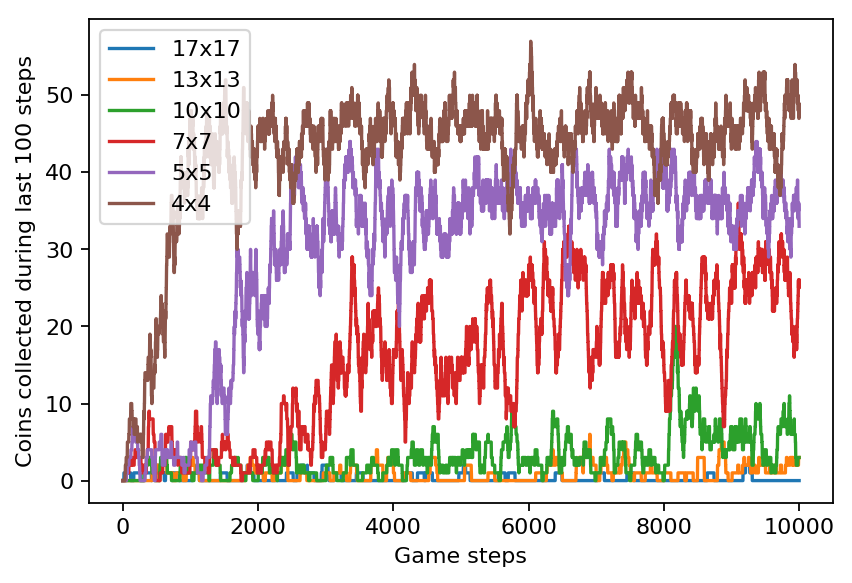
\includegraphics[width=\linewidth]{images/minigame-dense256-arch.png}
    \caption{Dense 256}
  \end{subfigure}
  \begin{subfigure}[b]{0.48\linewidth}
    \centering
    	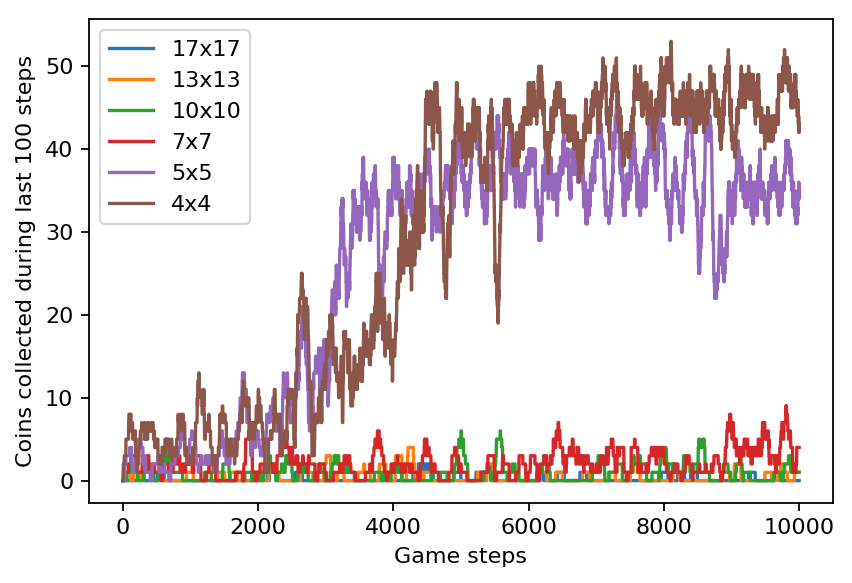
\includegraphics[width=\linewidth]{images/minigame-conv8-4-3-arch.png}
    \caption{Conv from Rainbow paper\cite{Hessel2018RainbowCI}}
  \end{subfigure}
  \quad
  \begin{subfigure}[b]{0.48\linewidth}
    \centering
      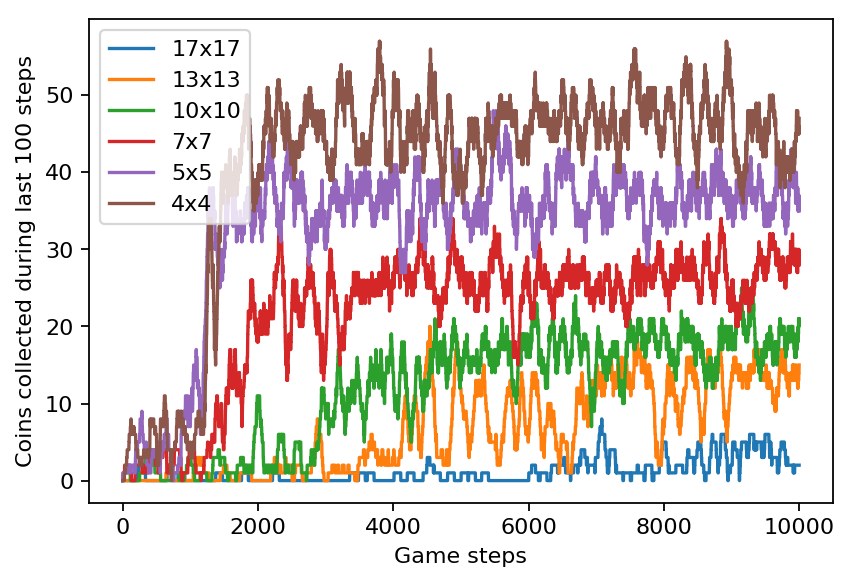
\includegraphics[width=\linewidth]{images/minigame-conv1-4-3-arch.png}
    \caption{Conv modified}
  \end{subfigure}
  \caption{Agents with different network architectures playing the minigame introduced in \ref{ch:minigame} for arena sizes from $4\times4$ to $17\times17$. There are three coins that can be collected per episode. The graphs show coins collected during the last 100 steps, continuing over episodes. For a big arena this number is naturally lower because of the large distances between coins, but it can be seen when and if the agent is plateauing.}
  \label{fig:networks}
\end{figure}


\begin{figure}
  \centering
  \begin{subfigure}[b]{0.48\linewidth}
    \centering
	\begin{tabular}{l l l}
		\multicolumn{3}{c}{Shared network} \\
		\midrule
		Dense & 64 units & relu \\
		Dense & 64 units & relu \\
		\toprule
		\multicolumn{3}{c}{Advantage / value stream} \\
		\midrule
		NoisyDense & 64 units & relu \\
		\toprule
	\end{tabular}
    \caption{Dense 64}
  \end{subfigure}
  \begin{subfigure}[b]{0.48\linewidth}
    \centering
	\begin{tabular}{l l l}
		\multicolumn{3}{c}{Shared network} \\
		\midrule
		Dense & 256 units & relu \\
		Dense & 256 units & relu \\
		\toprule
		\multicolumn{3}{c}{Advantage / value stream} \\
		\midrule
		NoisyDense & 256 units & relu \\
		\toprule
	\end{tabular}
    \caption{Dense 256}
  \end{subfigure}
  \caption{Simple fully connected (dense) network. The last value and advantage stream layer is omitted.}
  \label{fig:dense-arch}
\end{figure}


\begin{figure}
  \centering
  \begin{subfigure}[b]{0.48\linewidth}
    \centering
	\begin{tabular}{l l l l l}
		\multicolumn{5}{c}{Shared network} \\
		\midrule
		& $n_c$ & $f$ & $s$ & \\
		\midrule
		Conv2D & 32 & 8 & 4 & relu \\
		Conv2D & 64 & 4 & 2 & relu \\
		Conv2D & 64 & 3 & 1 & relu \\
		\toprule
		\multicolumn{5}{c}{Advantage / value stream} \\
		\midrule
		NoisyDense & \multicolumn{3}{l}{512 units} & relu \\
		\toprule
	\end{tabular}
    \caption{Conv from Rainbow paper\cite{Hessel2018RainbowCI}}
    \label{fig:conv-original}
  \end{subfigure}
  \begin{subfigure}[b]{0.48\linewidth}
    \centering
	\begin{tabular}{l l l l l}
		\multicolumn{5}{c}{Shared network} \\
		\midrule
		& $n_c$ & $f$ & $s$ & \\
		\midrule
		Conv2D & 32 & 1 & 1 & relu \\
		Conv2D & 64 & 4 & 2 & relu \\
		Conv2D & 64 & 3 & 2 & relu \\
		\toprule
		\multicolumn{5}{c}{Advantage / value stream} \\
		\midrule
		NoisyDense & \multicolumn{3}{l}{512 units} & relu \\
		\toprule
	\end{tabular}
    \caption{Modified convolutional NN}
    \label{fig:conv-modified}
  \end{subfigure}
  \caption{Convolutional network with number of channels $n_c$, filter size $f$ and stride $s$. The last value and advantage stream layer is omitted.}
  \label{fig:conv-arch}
\end{figure}

